

\subsection{Locality based overlay}

\begin{itemize}
	
	\item clustering
	
	\item Vivaldi + spirale

\end{itemize}

\subsection{Library for locality based algorithm}

%   * Construire des algos distribues fonctionnant en reseau est dur: couts 
% 	  impliques par la tolerance aux pannes et synchro.
%   * Ces couts sont parfois dus aux modeles de programmation.
Building a distributed algorithm that works at large scale is complex: fault
tolerance, synchronization and network overhead can have a cost that 
significantly impact on performance and scalability. This can be the result of a
bad software design, or the consequence of the use of an inapropriate 
programming model for a given situation, as sharing states in a distributed
context.

%   * La collaboration entre processus peut se faire de deux maniere:
%       A) partage d'etat.
%       B) echange de message.
This is especially true in situation where a process share a ressource with some 
other processes. This situation, also known as \emph{race condition situation}, 
has been thoroughly studied, which led to different ways to organize 
collaboration between concurrent actors that have to work concurrently:

\begin{description}

	\item [Shared state] : A ressource is shared between different processes: it
	requires that each process waits for its turn before acquiring it for use.
	This property can be guaranteed by using locks to control acces to shared
	ressource : processes have to wait that the ressource becomes free
	before using it.

	\item [Message passing] : Each process has its own state and collaborate
	with other processes by exchange of messages. In the case of the actor model 
	\cite{Hewitt1973}, a process becomes an \emph{actor} wich processes one
	message at a time. This is a lock free approach with no	shared state.

\end{description}

%   * les verrous sont des nids a deadlocks.
% 	* DVMS utilise le modele d'acteurs:
%		- chaque instance ne communique qu'avec des messages.
%		- on favorise les collaborations proches.
Locking ressources often leads to deadlock \cite{agha:1986}, which can have
a significant impact on performance and scalability. That is why we decided to
leverage the actor model to reoarganize DVMS: each instance will collaborate
by exclusively exchanging messages and priority will be given to collabarotion
between close instances.

%   * ainsi on a créé une librarie qui:
%		- favorise le dvlpt d'appli distribuée.
%		- se base sur des langages/frameworks modernes.
%	* la librairie se base sur la prog fonctionnelle et le peerActor.
With that in mind, we created a new library whose role is to ease the
development of distributed application: it is based on modern piece of software
(Scala and akka) based on the actor model. This library makes intensive use of
functionnal programming and the concept of \emph{peer actor}.

\subsubsection{Peer actor abstraction}

%   * Peer actor:
%		- apporte la tolerance aux pannes, abstraction du réseau, communication
%		  interservices.
%		- propose une API pour développer vite.
\emph{Peer actor} is an actor that provides several features: fault tolerance,
network abstraction, communication between services. It provides an API that 
enables the fast developement of distributed application : connection between
instances of the application is automatically maintained, meaning that all 
efforts can be concentrated on designing algorithms.

%   * Peer actor deux sous acteurs:
%		- notification actor: systeme a evenement pour les services.
%		- network overlay actor: réseau avec implémentation chord et vivaldi.
Peer actor contains two sub actors: \emph{notification actor} and \emph{network
overlay actor}. Notification actor enables services to subscribe to events that
will be triggered by other services. Network overlay actor is in charge of 
sending/receiving message through network. There exist two implementations of 
this network overlay actor: one is based on a Chord ring \cite{stoica2001chord},
while the other is based on vivaldi algorithm to leverage locality properties.

\begin{figure}[h!]
  \centering
  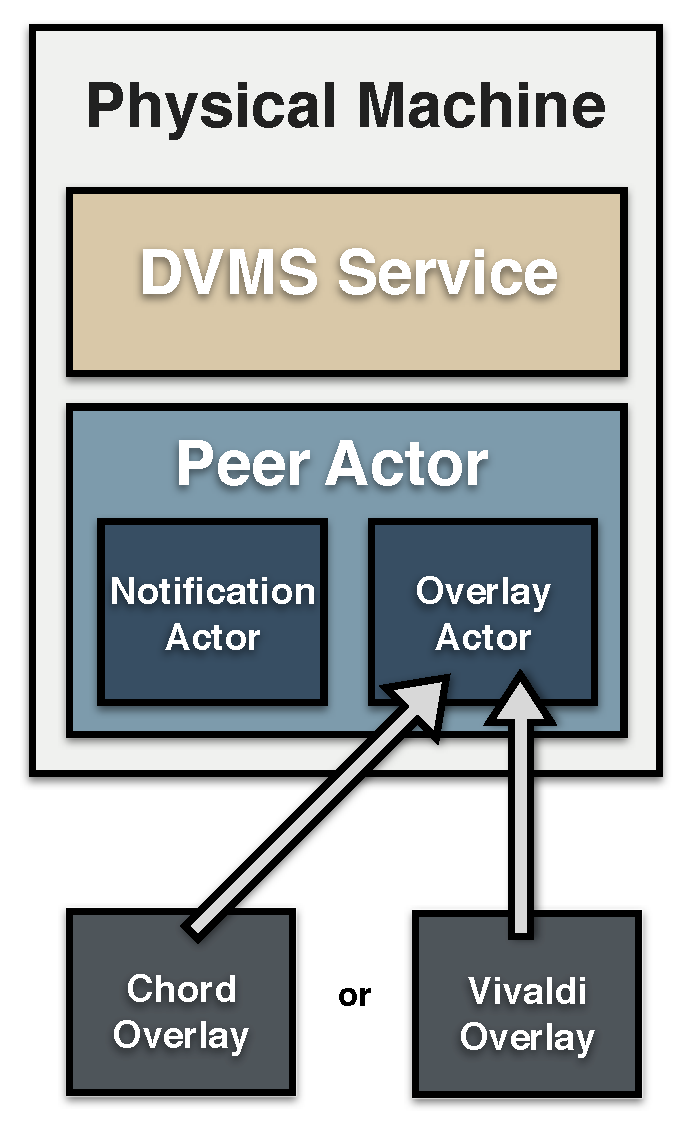
\includegraphics[width=0.5\linewidth]{Figures/DVMS.pdf}
  \caption{Architecture of DVMS based on peer actor.}%
  \label{fig:isp}%
\end{figure}

